%%%%%%%%%%%%%%%%%%%%%%%%%%%%%%%%%%%%%%%%%%%%%%%%%%%%%%%
%% Bachelor's & Master's Thesis Template             %%
%% Copyleft by Artur M. Brodzki & Piotr Woźniak      %%
%% Faculty of Electronics and Information Technology %%
%% Warsaw University of Technology, 2019-2020        %%
%%%%%%%%%%%%%%%%%%%%%%%%%%%%%%%%%%%%%%%%%%%%%%%%%%%%%%%

\documentclass[
    left=2.5cm,         % Sadly, generic margin parameter
    right=2.5cm,        % doesnt't work, as it is
    top=2.5cm,          % superseded by more specific
    bottom=3cm,         % left...bottom parameters.
    bindingoffset=6mm,  % Optional binding offset.
    nohyphenation=false % You may turn off hyphenation, if don't like.
]{eiti/eiti-thesis}

\langpol % Dla języka angielskiego mamy \langeng
\graphicspath{{img/}}             % Katalog z obrazkami.
\addbibresource{bibliografia.bib} % Plik .bib z bibliografią

\begin{document}

%--------------------------------------
% Strona tytułowa
%--------------------------------------
\MasterThesis % Dla pracy inżynierskiej mamy \EngineerThesis
\instytut{Instytut Automatyki i Informatyki Stosowanej}
\kierunek{Informatyka}
\specjalnosc{Inteligentne Systemy}
\title{
    Rozpoznawanie dyscypliny sportu na podstawie materiałów wideo
}
\engtitle{ % Tytuł po angielsku do angielskiego streszczenia
    Sport discipline classification based on video materials
}
\author{inż. Rafał Lewanczyk}
\album{293140}
\promotor{dr inż. Artur Wilkowski}
\date{\the\year}
\maketitle

%--------------------------------------
% Streszczenie po polsku
%--------------------------------------
\cleardoublepage % Zaczynamy od nieparzystej strony
\streszczenie
Rozpoznawanie dyscypliny sportu jest zadaniem klasyfikacji aktywności grupowych. Ma ono zastosowanie przy organizowaniu dużych zbiorów nagrań wideo w celu np. proponowanie treści, lub wyszukiwaniu po słowach kluczowych. 

W tej pracy przetestowane zostały podejścia do klasyfikacji aktywności grupowych poprzez analizę aktywności pojedynczych osób przy pomocy cech RGB lub cech szkieletowych, analizę cech RGB całych klatek nagrania oraz kombinacji tych metod. Opisane zostały szczegółowe architektury modeli oraz wnioski z ich działania. Dokonane zostało również porównanie z modelami bazowymi na badanym zbiorze. 

Efektem pracy jest model osiągający skuteczność wynoszącą 80.56\% na zbiorze danych SVW \cite{svw} oraz cały system przetwarzania wideo ekstrahujący wymagane cechy. 
\slowakluczowe sport, aktywności grupowe, percepcja maszyn, klasyfikacja

%--------------------------------------
% Streszczenie po angielsku
%--------------------------------------
\newpage
\abstract 
Recognizing sports disciplines is a task of classifying group activities. It is applied when organizing large sets of video recordings for purposes such as suggesting content or searching by keywords.

In this study, approaches to classify group activities were tested by analyzing the activities of individual persons using RGB features or skeletal features, analyzing the RGB features of entire frames of the recording, and combinations of these methods. Detailed architectures of the models and conclusions from their operation were described. Created models were compared to selected baseline models.

The result of the work is a model achieving an accuracy of 80.56\% on the SVW data set \cite{svw} and an entire video processing system extracting the required features.
\keywords sport, group activities, computer vision, classification

%--------------------------------------
% Oświadczenie o autorstwie
%--------------------------------------
\cleardoublepage  % Zaczynamy od nieparzystej strony 
\pagestyle{plain}
\makeauthorship
% TODO: END !!!!!!!!!!!!!!!!!!!!!!!!!!!!!

%--------------------------------------
% Spis treści
%--------------------------------------
\cleardoublepage % Zaczynamy od nieparzystej strony
\tableofcontents

%--------------------------------------
% Rozdziały
%--------------------------------------
\cleardoublepage % Zaczynamy od nieparzystej strony
\pagestyle{headings}

\newpage % Rozdziały zaczynamy od nowej strony.
\section{Wstęp}

\subsection{Problem}
Wraz z bardzo szybkim rozwojem technologii, smartfony oraz inne urządzenia przenośne stały się wszechobecne. Skutkiem tego jest stale rosnąca liczba danych wizualnych, takich jak zdjęcia oraz nagrania. Zgodnie z najnowszymi raportami firmy Sandvine\cite{sandvine}, aż 65\% całkowitego ruchu internetowego jest generowane właśnie przez treści wideo. Co więcej, przewiduje się, że ten odsetek będzie nadal rósł.

Semantyczny opis treści wideo umożliwia bardziej efektywne przeglądanie i wyszukiwanie ogromnych zbiorów, takich jak YouTube czy Instagram, dzięki lepszemu indeksowaniu i personalizacji treści. To pozwala użytkownikom odkrywać treści zgodne z ich zainteresowaniami, co zwiększa zaangażowanie i lojalność wobec platformy. Dzięki temu semantyczny opis przyczynia się do doskonalenia jakości usług i wzmocnienia konkurencyjności na rynku cyfrowym.

Klasyfikacja nagrań wideo może odbywać się na różnych poziomach. Na najwyższym poziomie można określić ogólną tematykę lub rodzaj przedstawionych treści, na przykład podział na kreskówki, sporty czy nagrania pochodzące z kamer monitoringu. Na kolejnym poziomie, działając w kontekście określonej klasy, można skupić się na konkretnych podklasach, np. dla nagrań sportowych dokonać klasyfikacji na konkretne dyscypliny, lub dla nagrań pochodzących z monitoringu podziału na sytuacje niebezpieczne oraz nie stanowiące zagrożenia. Istnieje również możliwość jeszcze bardziej szczegółowej klasyfikacji, gdzie dla każdego z nagrania określa się szczegółową akcję zawartą w jego fragmencie. W przypadku dyscyplin sportowych mogą to być konkretne akcje, z których składają się dane sporty, takie jak serwisy, odbiory, uderzenia forehandowe czy backhandowe w tenisie, a także ataki i bloki w siatkówce. 

\subsection{Zastosowania}
Tego typu systemy mają niezwykle szerokie zastosowanie zarówno w przetwarzaniu danych strumieniowych w czasie rzeczywistym, jak i w analizie wcześniej przygotowanych zbiorów. Przykładowe zastosowania systemów klasyfikacji akcji:
\begin{itemize}
    \item Etykietowanie zbiorów danych wideo, w celu ułatwienia wyszukiwania oraz serwowania treści dopasowanych do zainteresowań użytkownika
    \item Wyszukiwanie kluczowych elementów w rozgrywce sportowej, takich jak strzelenie bramki, skuteczny atak. Znajdowanie tego typu akcji pozwala na ich głębszą analizę oraz wytwarzanie skrótów meczów
    \item Aplikacje mające na celu poprawienia techniki wykonywanych sportów. W tym przypadku model może specjalizować się w rozpoznawaniu pojedynczych dyscyplin oraz rozpoznawać w jakim stopniu wykonywana czynność jest zbliżona do tej samej czynności wykonywanej przez specjalistę. 
    \item Rozpoznawanie na żywo niebezpiecznych sytuacji w nagraniach pochodzących z kamer monitoringu, oraz informowanie w takich przypadkach służb specjalnych 
\end{itemize}
\subsection{Cel}
Celem projektu jest wytworzenie systemu potrafiącego na podstawie nagrania wideo określić, jaką przedstawia ono dyscyplinę sportu. 
         % Wygodnie jest trzymać każdy rozdział w osobnym pliku.
\newpage % Rozdziały zaczynamy od nowej strony.
\section{Przegląd literatury}
Problem rozpoznawania dyscypliny sportu jest pod-problemem rozpoznawania aktywności. Rozpoznawanie aktywności można podzielić na trzy poziomy \cite{Wu2021}:
\begin{itemize} 
\item Aktywności indywidualne -  skupiające się na czynnościach wykonywanych przez jedną osobę. W takim kontekście, szczegółowe cechy sylwetki oraz dynamika ruchu ciała dostarczają wystarczających danych do precyzyjnej klasyfikacji.
\item Aktywności grupowe - dotyczą akcji, w których możemy rozróżnić indywidualne sylwetki, ale ich czynności nie są do końca jednoznaczne. W takim przypadku musimy uwzględnić interakcje pomiędzy uczestnikami oraz spojrzeć na całość sytuacji, nie skupiając się tylko na indywidualnych ruchach
\item Aktywności tłumu - brak możliwości analizowania indywidualnych osób,  należy patrzyć na akcje jako całość
\end{itemize}
Klasyfikacja dyscyplin sportowych jest kombinacją klasyfikacji aktywności indywidualnych oraz grupowych. 

Problem rozpoznawania aktywności jest badany już od długiego czasu, jednak w dużej mierze opiera się on na badaniu aktywności indywidualnych. Skupia się on na wykorzystywaniu ręcznie zaprojektowanych cech. Rozpowszechnienie się uczenia głębokiego otworzyło nowe możliwości w tej dziedzinie, a modele oparte na tej metodzie osiągają dotychczas najlepsze skuteczności. W tym rozdziale omówione zostaną prace istotne lub podobne do tej.  

\subsection{Modele hierarchiczne uczenia głębokiego}
Modele hierarchiczne opierają się na założeniu, że aby zrozumieć aktywność grupową, konieczne jest indywidualne analizowanie akcji każdej z poszczególnych osób. Wynikowa aktywność jest efektem klasyfikacji wartości funkcji agregującej cechy poszczególnych osób. To podejście wymaga intensywnego wstępnego przetworzenia nagrania, które obejmuje identyfikację poszczególnych osób, śledzenie ich detekcji w sekwencji, a także ekstrakcję unikalnych cech tych osób, takich jak cechy szkieletowe czy cechy RGB.
\subsubsection{Hierarchiczne modele splotowe}
Fabio Zappardino et al.\cite{Szkielety} w swojej pracy proponuje podejście oparte na cechach sylwetkowych poszczególnych osób oraz kombinacji ich przy pomocy sieci splotowych CNN. Zaproponowana w pracy architektura składa się z trzech gałęzi o identycznej strukturze, ale oddzielnych wagach, gdzie każda z gałęzi modelu przyjmuje na wejściu ręcznie wyselekcjonowane cechy, oparte na danych szkieletowych wyekstrahowanych przy pomocy modelu OpenPose \cite{openpose}. Przyjmowane cechy to: 
\begin{itemize}
    \item Ruch wyrażony poprzez skonkatenowane wektory przedstawiające pozy w kolejnych klatkach jednej osoby 
    \item Ruch wyrażony poprzez wyliczenie przesunięcia każdego z wyznaczonych stawów
    \item Zależność do pozostałych członków grupy, poprzez wyliczenie różnicy stawów między analizowanym uczestnikiem, a wybranym dla akcji uczestnikiem centralnym
\end{itemize}
Wyjścia z sieci splotowych są konkatenowane oraz trafiają do kolejnej warstwy splotowej, której odpowiedzialnością jest zakodowanie ruchu poszczególnych osób.

Tego typu przetwarzanie zostaje nałożone na każdą z osób biorącą udział w aktywności oraz zebrane do wspólnej macierzy, na którą nałożona zostaje transformacja MaxPooling'u po osobach. Tak przetworzona macierz trafia do modelu klasyfikującego. Architektura całego systemu została przedstawiona na rysunku \ref{fig:szkielety-arch}.
\begin{figure}[!h]
    \centering 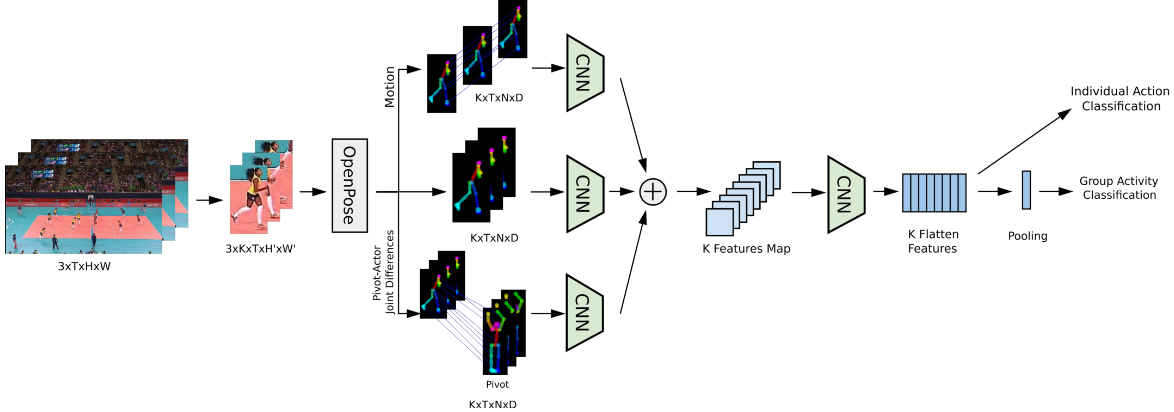
\includegraphics[width=0.9\linewidth]{szkielety.png}
    \caption{Hierarchiczny model oparty na sieciach splotowych oraz cechach szkieletowych}
    \label{fig:szkielety-arch}
\end{figure}

W pracy przetestowane zostały dwa podejścia do treningu modelu: 
\begin{itemize}
    \item Rozłączny trening modelu działającego na pojedynczych osobach oraz klasyfikatora. W tym przypadku wymagana są etykiety akcji poszczególnych osób, autor wypróbował również wygenerowanie własnych etykiet poprzez klastrowanie wyjść z wcześniej wytrenowanego już modelu P3D
    \item Trening całościowy modelu
\end{itemize}
Testy przeprowadzone zostały na zbiorze danych, składającym się z nagrań zagrań w siatkówce \cite{Ibrahim2015}, osiągając najlepszą skuteczność dla całościowego treningu modelu wynoszącą 91\%. 

\subsubsection{Hierarchiczne modelowanie czasowe} 
Ibrahim et al. \cite{Ibrahim2015} zaproponował w swojej pracy hierarchiczny model oparty na sieciach LSTM oraz cechach RGB wyekstrahowanych przy pomocy wcześniej wytrenowanej sieci AlexNet \cite{alexnet}. 

Architektura modelu składa się z dwóch sieci LSTM, połączonych w hierarchię. Zdaniem pierwszej z sieci jest analiza aktywności indywidualnej. Jest ona nakładana na każdą z osób wykrytych w akcji. Sieć składa się z 9 kroków czasowych oraz 3000 stanów ukrytych, na wejściu otrzymuje sekwencje składającą się z cech RGB poszczególnej osoby, na wyjściu zwracane są wszystkie stany ukryte ostatniej warstwy LSTM sieci. Następnie wykonana zostaje transformacja MaxPooling'u stanów ukrytych po osobach, która jest wejściem do kolejnego modelu LSTM składającego się z 9 kroków czasowych oraz 500 stanów ukrytych. Architektura modelu została przedstawiona na rysunku \ref{fig:ibrahim-arch}. 
\begin{figure}[!h]
    \centering 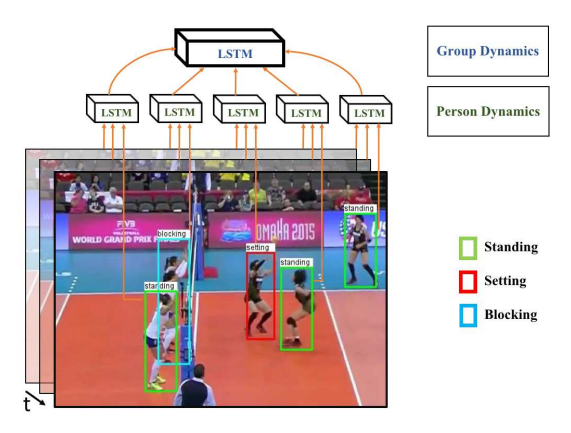
\includegraphics[width=0.9\linewidth]{ibrahim.png}
    \caption{Hierarchiczny model oparty na sieciach LSTM oraz cechach RGB}
    \label{fig:ibrahim-arch}
\end{figure}
Trening modeli został przeprowadzony osobno dla każdej z sieci w hierarchii. Dla modelu niższego stopnia wykorzystane zostały etykiety aktywności indywidualnych. Trening modelu wyższego poziomu odbywa się przy zamrożeniu wag modelu niższego poziomu, wykorzystuje już docelowe etykiety aktywności grupowych. 

Model osiąga skuteczność 81.5\% na zbiorze danych Collective Activity Dataset \cite{collective_ds}, jednak dla bardziej złożonych zbiorach danych radzi sobie gorzej, osiągając skuteczność wynoszącą 51.1\% na zbiorze danych zagrań w siatkówce \cite{Ibrahim2015}.

\subsection{Modele oparte na cechach całego obrazu}
Charakterystyczną cechą tego podejścia jest zaawansowana analiza klatek nagrania. Transformuje ono zagadnienie klasyfikacji aktywności grupowej w ogólny problem klasyfikacji wideo, gdzie liczba osób na nagraniu nie ma znaczenia. Może to być jedna osoba, grupa, tłum, a nawet brak osób. Dzięki temu nie wymaga ono tak intensywnego wstępnego przetworzenia danych i jest bardziej oszczędne obliczeniowo. 

\subsubsection{Dwukierunkowy model LSTM oparty na cecach RGB}
Ullah A. et al. \cite{Ullah2017} w swojej pracy proponuję podejście, które polega na ekstrakcji cech RGB za pomocą sieci splotowych oraz kodowaniu sekwencji za pomocą dwóch wzajemnie połączonych warstw LSTM, która następnie podlega klasyfikacji. Architektura rozwiązania została przedstawiona na rysunku \ref{fig:ullah-arch}
\begin{figure}[!h]
    \centering 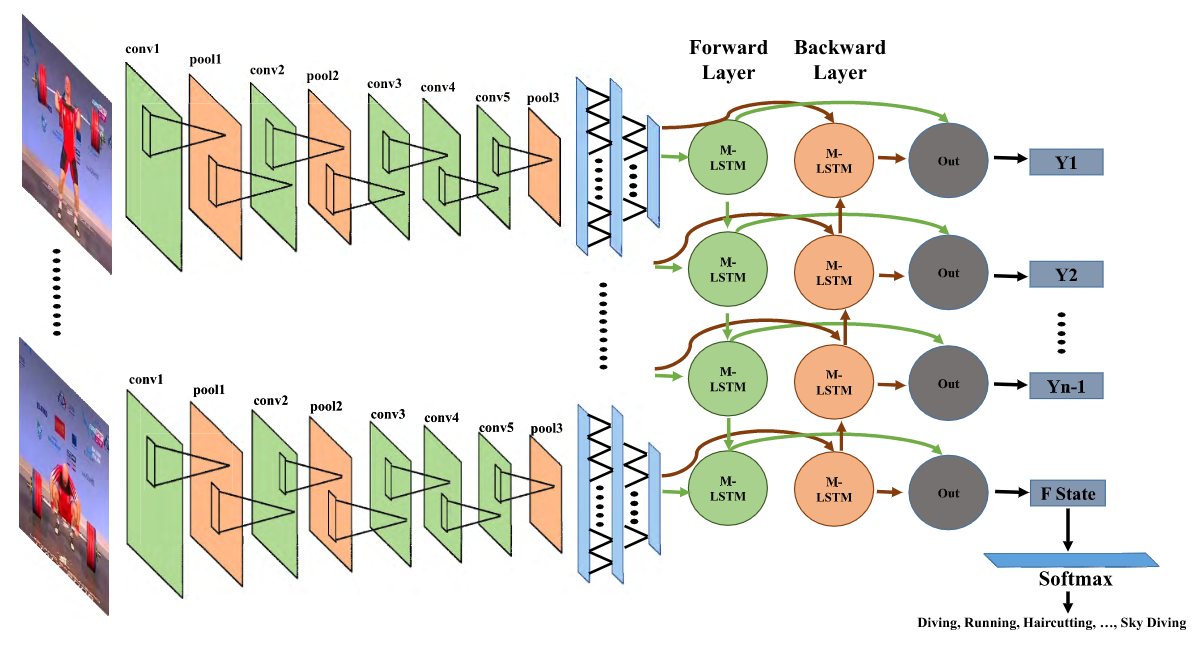
\includegraphics[width=0.9\linewidth]{ullah.png}
    \caption{Dwukierunkowy model LSTM oparty na cechach RGB}
    \label{fig:ullah-arch}
\end{figure}
Model klasyfikuje nagrania sekunda po sekundzie, wybierając z każdej sekundy co 6 klatkę. Został przetestowany na zbiorze danych wideo pochodzących z serwisu YouTube \cite{yt_dataset}, osiągając skuteczność 92.84\%. 

\subsection{Rozwiązania komercyjne}
\subsubsection{AutoML} 
Na rynku dostępne są narzędzia pozwalające na wytworzenie modelu uczenia maszynowego o dowolnym zastosowaniu (m.in. klasyfikacja aktywności), bez konieczności projektowania architektury. Przykładem takiego narzędzia jest AutoML (Automated Machine Learning)\cite{automl} firmy Google. 

Podejście to opiera się na wybraniu zadania jakie ma realizować model (jaki typ danych model otrzyma na wejściu, jaki ma być rezultat modelu np. klasyfikacja). Następnie proces w oparciu o analizowany zbiór danych oraz udostępnione informacje automatycznie wybiera odpowiedni typ modelu uczenia maszynowego, który najlepiej pasuje do określonego problemu. Po wyborze modelu, proces AutoML trenuje go, dopasowując parametry i wagi do danych treningowych, wykonuje automatycznego wyszukania architektury (NAS), dokonuje optymalizacji modelu, wybierając optymalne parametry i techniki regularyzacji. Proces zwraca najlepszy znaleziony model. 

Ze względu, że jest to zastosowanie komercyjne, szczegółowe informacje na temat działania modelu nie są publicznie dostępne.    % Umożliwia to również łatwą migrację do nowej wersji szablonu:
\newpage
\section{Proponowane rozwiązanie}
\subsection{Architektura systemu}

\subsection{Klasyfikacja}\label{klasyfikacja}
W celu dokonania klasyfikacji, z każdego nagrania wybrane zostają 3 sekwencje, składające się z 64 kolejnych klatek.
Rozkład wybranych sekwencji dokonany jest w taki sposób, aby były one rozłożone możliwie równomiernie. W przypadku gdy
długość
3 sekwencji przekracza długość nagrania, sekwencje mają części wspólne, w przeciwnym przypadku będą rozłączne.
Przykładowy podział na sekwencje został przedstawiony na rysunku \ref{fig:sekwencje}. Zaprezentowane w pracy modele
dokonują klasyfikacji sekwencji. Klasy nagrań zostają wybrane poprzez zsumowanie przewidzianych przez model
prawdopodobieństw dla każdej z sekwencji oraz wybranie klasy o największym prawdopodobieństw.
\begin{figure}[!h]
    \centering 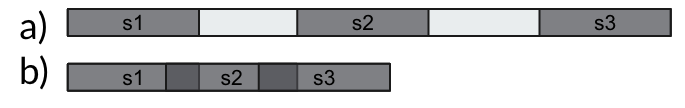
\includegraphics[width=0.75\linewidth]{sekwencje.png}
    \caption{Rozkład wybieranych sekwencji, a) łączna długość sekwencji mniejsza niż długość nagrania, b) łączna długość wybranych sekwencji przekracza długość nagrania - sekwencje mają części wspólne}
    \label{fig:sekwencje}
\end{figure}
\subsection{Wykorzystane cechy}
W pracy wykorzystane zostały trzy rodzaje cech wyekstrahowanych z klatek nagrania. Wykorzystane cechy zostały zwizualizowane na rysunku \ref{fig:wiz-cech}

Modele hierarchiczne biorące pod
uwagę aktywności wyselekcjonowanych osób wymagają dodatkowego przetworzenia wideo składającego się z następujących
kroków: \begin{itemize}
\item Detekcja osób w nagraniu
\item Śledzenie wykrytych osób
\end{itemize}
\begin{figure}[!h]
    \centering 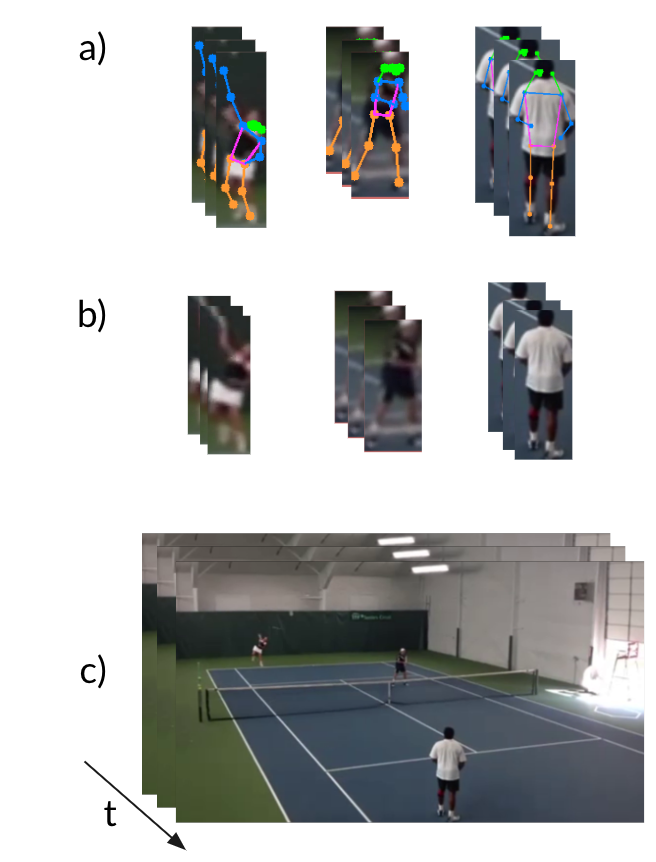
\includegraphics[width=0.70\linewidth]{features-vis.png}
    \caption{Wizualizacja cech użytych do reprezentacji sekwencji. a) cechy szkieletowe, b) cechy RGB pojedynczych osób, c) cechy RGB całego obrazu}
    \label{fig:wiz-cech}
\end{figure}
\subsubsection{Cechy szkieletowe}
Cechy szkieletowe wyekstrahowane zostały przy pomocy modelu YOLOv7-pose \cite{yolov7-pose}, z wycinków klatek
zawierających pojedyncze osoby. Sekwencja składająca się z cech szkieletowych reprezentowana jest przez wektor o
wymiarach $(N, T, 17, 2)$, gdzie pierwszy wymiar $N$ oznacza ilość osób na wejściu do modelu, $T$ liczbę badanych klatek,
natomiast 2 ostatnie wymiary oznaczają 17 dwuwymiarowych punktów reprezentujących szkielet.
\subsubsection{Cechy RGB pojedynczych osób}
Cechy RGB pojedynczych osób, wyekstrahowane zostały przy pomocy modelu mobilenet\cite{mobilenet}, zakończonego warstwą
AveragePooling'u z wycinków klatek zawierających pojedyncze osoby. Sekwencja składająca się z cech RGB pojedynczych
osób, reprezentowana jest przez wektor o wymiarach $(N, T, 256)$, gdzie $N$ oznacza ilość osób na wejściu do modelu, $T$ liczbę badanych klatek, 256 to rozmiar wektora zakodowanych cech RGB wyznaczonych przez model mobilenet zredukowany przy
pomocy algorytmu analizy głównych składowych PCA z oryginalnego wymiaru wynoszącego 960.  
\subsubsection{Cechy RGB całego obrazu}\label{sekwncje-klatek}
Cechy RGB całego obrazu, wyznaczone zostały przy pomocy tej samej metody co w przypadku pojedynczych osób, różnią
się tylko tym, że badany jest cały obraz zamiast pojedynczej osoby. Tego typu sekwencja reprezentowana jest przez wektor
o wymiarach $(T, 256)$, gdzie $T$ oznacza liczbę badanych klatek, 256 to rozmiar wektora RGB ~
\subsection{Hiper-parametry sekwencji}
\subsubsection{Liczba osób na wejściu do modelu}\label{kryteria-wyboru}
Liczba osób na wejściu do modelu,
reprezentowana w ww. wektorach przez literę $N$, w przeprowadzonych eksperymentach wynosi 6. Wartość ta wyznaczona została
poprzez wyliczenie średniej ilości wykrytych osób we wszystkich przetworzonych klatkach w całym zbiorze danych. Parametr ten ma również duże znaczenie na rozmiar danych treningowych modelu. 

Aby osoba mogła zostać zaliczona do sekwencji, musi znajdować się w co najmniej 70\% klatek sekwencji. Warunek ten 
wynika z możliwości wystąpienia następujących sytuacji: \begin{itemize} 
\item Osoba może pojawić się w polu widzenia kamery dopiero pod koniec sekwencji np. wbiec
\item Detektor może zgubić ślad osoby
\item Poruszająca się kamera, śledząca akcje może uchwycić chwilowo osobę stojącą w tle 
\end{itemize} 
W powyższych przypadkach istnieje duże prawdopodobieństwo, że taka osoba nie wnosi informacji o dziejącej się akcji i może stanowić 
tylko szum na wejściu modelu. W przypadku, gdy wykryta osoba spełnia ten warunek, ale nie występuje na wszystkich 
klatkach badanej sekwencji, jej brakujące klatki zostają uzupełnione poprzez powielenie najbliższej dostępnej klatki. 

W ten sposób przetworzony 
zbiór wykrytych osób zostaje posortowany w ramach ich sekwencji według ich największego otaczającego prostokąta, oraz 
z pierwszych $N$ osób zostaje zbudowany wektor wejściowy. Tego typu sortowanie ma na celu wybranie osób na pierwszym  
planie, który najprawdopodobniej niesie najwięcej informacji o odbywającej się akcji. 

W przypadku, gdy w sekwencji bierze udział mniej niż N osób, brakująca część wektora zostaje uzupełniona zerami. Badane
są tylko sekwencje, w których występuje co najmniej jedna osoba. 

\subsubsection{Długość sekwencji}
Długość sekwencji $T$ oznacza liczbę klatek przedstawiających akcje, z których zostały wyekstrahowane cechy. W pracy przyjęta została wartość 64, jako że wszystkie nagrania w badanym zbiorze danych składają się z częstotliwości 30 klatek na sekundę badane są sekwencje około 2 sekundowe. Sekwencje budowane są z następujących po sobie klatkach. 

\subsection{Architektura systemu}
Architektura systemu klasyfikującego, razem ze wstępnym przetworzeniem danych oraz wykorzystanymi modelami została przedstawiona na rysunku \ref{fig:architektura}.

Na wejściu system przyjmuje surowe, nieprzetworzone w żaden sposób nagranie, które podawane jest procesowi ekstrakcji cech. Etap ten na rysunku \ref{fig:architektura} został zaznaczony liniami przerywanymi, ze względu na to, że jest on wymagany tylko w przypadku, gdy model klasyfikujący bierze pod uwagę akcje pojedynczych osób (modele hierarchiczne), dla modelu badającego cechy całego obrazu krok ten może zostać pominięty. Dysponując tak przetworzonymi danymi, wybierane są sekwencje nagrania, które są wejściami do klasyfikatora.
\begin{figure}[!h]
    \centering 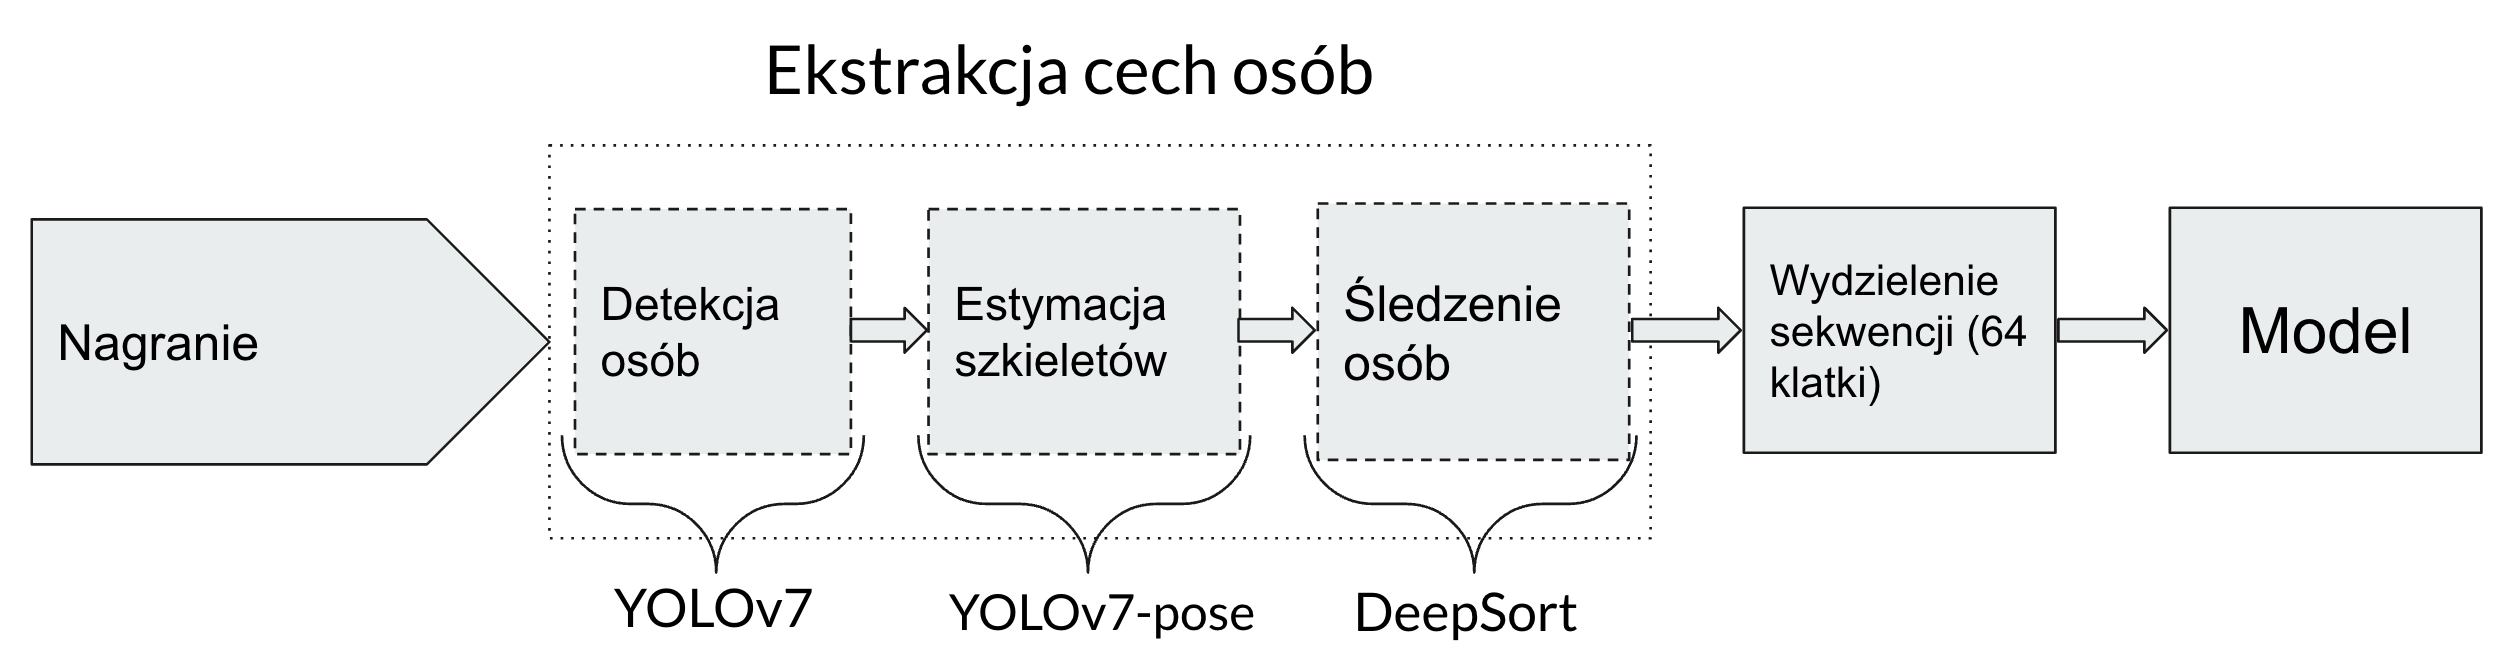
\includegraphics[width=0.90\linewidth]{architektura.png}
    \caption{Graf przedstawiający architekturę systemu}
    \label{fig:architektura}
\end{figure}
\subsubsection{Detekcja osób oraz estymacja szkieletów}
Detekcja osób w nagraniu odbywa się przy pomocy modelu YOLOv7 \cite{yolov7}. Jest to najlepszy dostępny detektor,
dostępny na moment implementacji systemu. Jego główna zaleta polega na tym, że wykonuje cały proces detekcji jednocześnie, bez potrzeby wielokrotnego analizowania obrazu, co sprawia, że jest bardzo szybki. YOLO dzieli obraz na siatkę komórek i dla każdej komórki przewiduje obiekt znajdujący się wewnątrz niej. Dodatkowo, model generuje otaczające prostokąty, które opisują położenie oraz wymiary wykrytych obiektów. Każdy prostokąt reprezentuje jedną detekcję.

Do estymacji szkieletów został również użyty model YOLOv7 dostosowany do do tego konkretnego zadania
\subsubsection{Śledzenie wykrytych osób}
Śledzenie wykrytych osób zostało wykonane przy użyciu algorytmu sortowanie głębokiego DeepSort. Algorytm ten dysponując detekcjami osób oraz ich cechami RGB wyznaczonymi przy pomocy detektora wykorzystuje algorytm SORT do przyporządkowania obiektów z bieżącej klatki do wcześniejszych identyfikowanych obiektów (jeśli istnieją) na podstawie odległości między cechami. SORT jest algorytmem śledzenia opartym na filtrze Kalmana, który estymuje pozycję i prędkość obiektów oraz śledzi je w czasie rzeczywistym.
Algorytym ten został wybrany ze względu na jego bardzo wysokie wyniki w rankingach algorytmów rozwiązujących śledzenie osób w grupie.
W implementacji systemu została użyta gotowa implementacja \cite{deepsort} algorytmu.
\subsection{Trening}
\subsubsection{Epoki oraz serie danych}
Modele trenowane są przez 50 epok, z warunkiem szybszego przerwania treningu: \textit{przerwij jeżeli funkcja straty nie spadła w przeciągu 3 ostatnich epok}. 

Serie danych, po których następuje aktualizacja wag modelu, została dobrana automatycznie przez bibliotekę Keras. 
\subsubsection{Funkcja celu}
Optymalizowana przez model funkcja celu jest wyrażona przez entropię krzyżową $L(y, \hat{y})$, gdzie $y$ oznacza przewidzianą dyscyplinę, a $\hat{y}$ jest prawdziwą wartością. 
\subsubsection{Optymalizator} 
Do nauki parametrów sieci neuronowej wykorzystany został stochastyczny spadek gradientu ADAM zaimplementowany w bibliotece Keras. Eksperymenty zostały wykonane przy stałych hiperparametrach wynoszących: 

$\eta=0.001, \ \ \beta_1=0.9,\ \  \beta_2=0.999$
\subsection{Zbiór danych}
Eksperymenty przeprowadzone zostały na zbiorze danych Sports Videos In The Wild. Zbiór składa się z nagrań
przedstawiających osoby uprawiające sporty, nagrane przez trenerów w warunkach treningowych, przez co mocno różnią się
one od typowych transmisji sportowych. Przykładowe klatki nagrań zostały przedstawione na rysunku \ref{fig:svw-klatki}.
Nagrania charakteryzują się dużą wariancją między klasową, która wynika ze zróżnicowanego tła, niereprezentatywnego
otoczenia, mocno zróżnicowanego wyposażenia sportowców oraz akcji wykonywanych zarówno przez profesjonalistów, jak i
amatorów.

Nagrania pochodzą z urządzen mobilnych trenerów, czego skutkiem jest różna rozdzielczość, kąt ustawienia
kamery, nieprzewidywalne ruchy kamery oraz różna długość nagrań zaczynając od 1.17 aż do 390.27 sekund.
\begin{figure}[!h]
    \centering 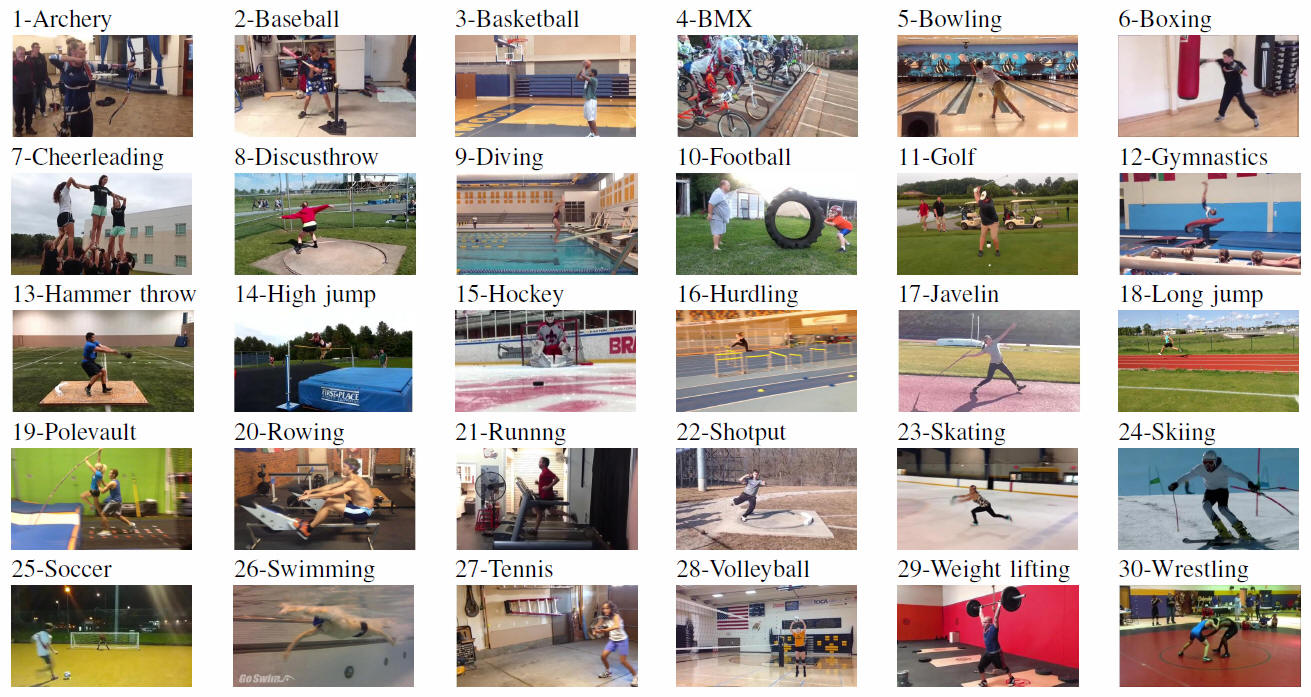
\includegraphics[height=8cm, width=0.99\linewidth]{svw-klatki.jpg}
    \caption{Klasy wraz z przykładowymi klatkami zbioru SVW}
    \label{fig:svw-klatki}
\end{figure}
\subsubsection{Statystyki zbioru}
Zbiór składa się łącznie z 4100 nagrań oraz 30 klas dyscyplin sportowych. Łączna długość nagrań wynosi 17.8 godzin. Rozmiary
poszczególnych klas zostały przedstawione na rysunku \ref{fig:raw-class-histogram}.
Twórcy zbioru danych dostarczyli również wyniki przeprowadzonych na zbiorze eksperymentów dla problemu rozpoznawania
dyscypliny sportu, jako metrykę bazową wynoszącą 61.53\%. Wynik ten został otrzymany przy pomocy kombinacji histogramów
zorientowanych gradientów (HOG), deskryptorów ruchu oraz deskryptorów trajektorii.
\begin{figure}[!h]
    \centering 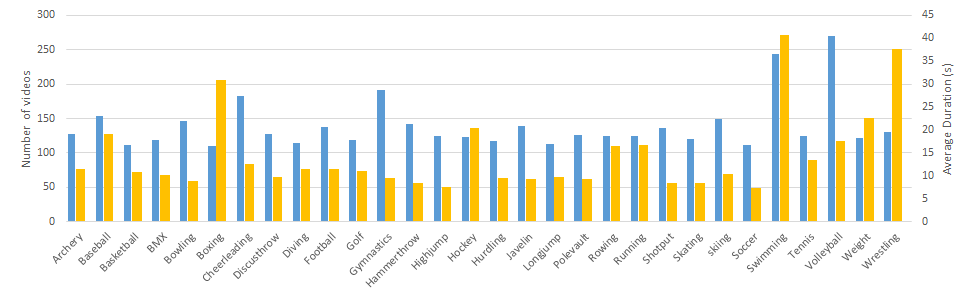
\includegraphics[width=0.90\linewidth]{stat1.png}
    \caption{Graf przedstawiający architekturę systemu}
    \label{fig:raw-class-histogram}
\end{figure}
\subsection{Ewaluacja modeli}
Zbiór danych SVW jest dostarczony razem z zalecanym podziałem przeznaczonym do walidacji krzyżowej o współczynniku
podziału wynoszącym $k = 3$. Metryki przedstawiające skuteczność modelu zostały wyznaczone przy pomocy podziału
zaproponowanego przez twórców zbioru składającego się z 70\% nagrań w zbiorze treningowym oraz 30\% nagrań w zbiorze testowym. 



  
\newpage
\section{Przeprowadzone eksperymenty}

\subsection{Hierarchiczny model szkieletowy}
Dysponując sekwencjami prześledzonych szkieletów występujących w nagraniu, gdzie sekwencja składa się z 6 osób, wybranych poprzez kryteria opisanych w rozdziale \ref{kryteria-wyboru}, pojedyncza sekwencja podawana jest na wejście modelu, gdzie każdej z osób odpowiada oddzielne wejście. Wszystkie sekwencje przetwarzane są równolegle przez warstwy LSTM, o współdzielonych wagach, mające na celu zakodowanie ruchów uczestników akcji. Warstwy LSTM zwracają wszystkie $T$ stany ukryte, które poddawane są transformacji MaxPooling'u po osobach, redukując jeden z wymiarów. Intuicją stojącą za zastosowaniem transformacji MaxPooling'u jest znalezienie ekstremalnych, wystających ponad normę czynności. Następnie zredukowane o wymiar ilości osób, stany ukryte LSTM trafiają do kolejnej warstwy LSTM kodującej globalną sekwencję, której wyjście trafia do warstwy gęstej oraz warstwy gęstej klasyfikującej. Opisana architektura jest reimplementacją architektury opisanej przez Ibrahima et. al \cite{Ibrahim2015}, dostosowaną do działania na wejściach składających się z sylwetek zamiast cech RGB. 

Przeprowadzone eksperymenty na architekturze pokazały, że zastąpienie pojedynczej warstwy LSTM kodującej globalnie sekwencje, takimi samymi dwiema warstwami LSTM połączonymi dwukierunkowo poprawia wyniki. Architektura modelu wraz z wymiarami wektorów wyjść została przedstawiona na rysunku \ref{fig:skeletons-arch}. Całkowita ilość trenowalnych parametrów modelu wynosi 435710. 
\begin{figure}[!h]
    \centering 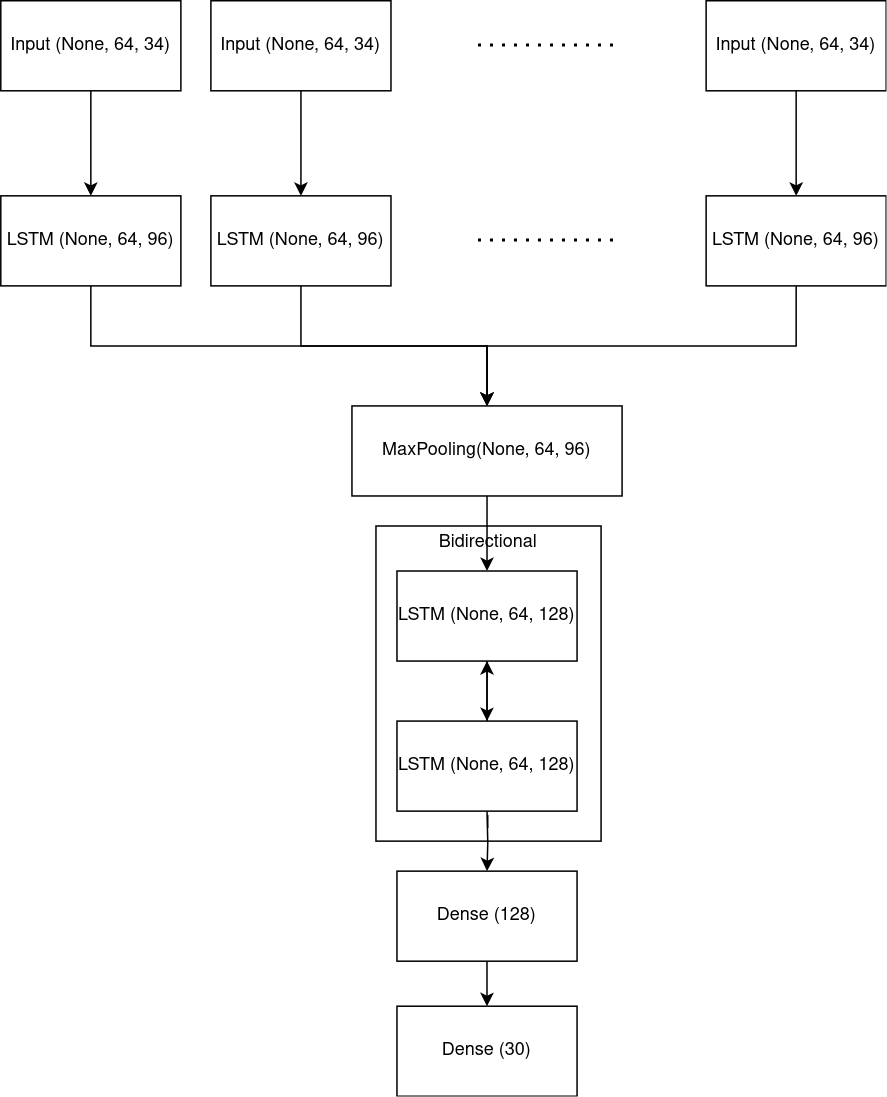
\includegraphics[width=0.70\linewidth]{skeletons-arch.png}
    \caption{Architektura hierarchicznego modelu czasowego opartego o szkielety uczestników akcji, z warstwą dwukierunkową LSTM}
    \label{fig:skeletons-arch}
\end{figure}

\subsubsection{Wyniki} 
Skuteczność hierarchicznego modelu opartego na cechach szkieletowych wyniosła 41.52\% , wyliczona w tabeli \ref{tab:szkielety-wyniki}. Na tak niską skuteczność składa się kilka czynników: \begin{itemize}
    \item Same szkielety niosą informację tylko i wyłącznie o ruchach poszczególnych osób, tracony jest cały pozostały kontekst akcji tj. tło, ubiór, sprzęt.
    \item Czynności wykonywane w sporcie mają bardzo duży wspólny podzbiór ruchów np. aktywność biegania występuje w prawie wszystkich sportach lekkoatletycznych. 
    \item W danych szkieletowych wyekstrahowanych przez model występuje szum związany z trudnością przetworzenia nagrań, do których dochodzą niestandardowe dla modelu pozy występujące w sporcie. 
\end{itemize}
\begin{table}[!h]  \centering
\caption{Wyniki modelu opartego na cechach szkieletowych}
\begin{tabular} {| c | c | c | c | r |} \hline
    Model & Podział 1.  & Podział 2. & Podział 3. & \textbf{Średnia} \\ \hline\hline
    Hierarchiczny model szkieletowy &  39.81\%	& 42.72\%	& 42.03\% & \textbf{41.52\%} \\ \hline
\end{tabular}
    \label{tab:szkielety-wyniki}
\end{table}
Ze względu na niską skuteczność modelu, badania modeli opartych wyłącznie na cechach szkieletowych zostały porzucone. 

\subsection{Hierarchiczne modele RGB}
\subsubsection{Hierarchiczny model RGB z warstwą MaxPoolingu}
Hierarchiczny model oparty na cechach RGB, oparty jest na tych samych założeniach oraz tej samej architekturze co model szkieletowy, różni się jedynie wejściem modelu, zamiast szkieletów działa na cechach RGB wyekstrahowanych przy pomocy modelu MobileNetV3 \cite{mobilenet}. Wraz ze zmianą wejścia konieczne jest również dostosowanie rozmiarów warstw. Architektura jest reimplementacją architektury przedstawionej w pracy Ibrahim et al. \cite{Ibrahim2015}, zmienione uległy wielkości warstw, ponieważ wektory wejściowe zostały uzyskane w inny sposób. Dla danej architektury, tak samo jak dla cech szkieletowych lepsze wyniki dało zastąpienie pojedynczej warstwy LSTM  dwoma warstwami połączonymi dwukierunkowo dla kodowania sekwencji. Architektura modelu została przedstawiona na rysunku \ref{fig:sp-arch}. Całkowita ilość trenowalnych parametrów modelu wynosi 450 974. 
\begin{figure}[!h]
    \centering 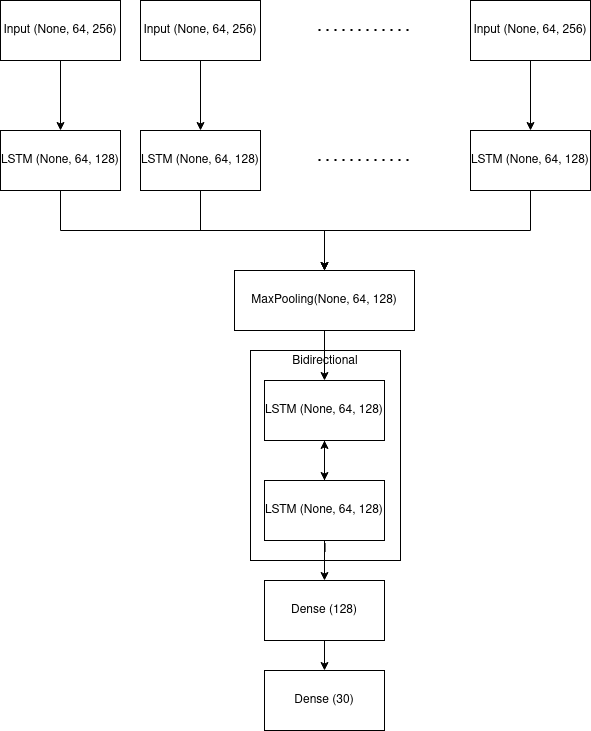
\includegraphics[width=0.70\linewidth]{sp-arch.png}
    \caption{Architektura hierarchicznego modelu czasowego opartego o cechy RGB uczestników akcji, z warstwą dwukierunkową LSTM}
    \label{fig:sp-arch}
\end{figure}

\subsubsection{Hierarchiczny model RGB z warstwą konkatenacji}
Przetestowana została również autorska modyfikacja modelu hierarchicznego. Eksperyment polegał na zastosowaniu dwóch dwukierunkowych warstw LSTM do zakodowania sekwencji pojedynczych osób oraz zastąpieniem warstwy MaxPooling'u warstwą konkatenacji. Pierwsza zmiana wynikała z obserwacji dokonanej w trakcie treningu, mówiącej, że dwukierunkowy LSTM daje lepsze wyniki dla zadania kodowania sekwencji aktywności. Druga zmiana wynikała z wątpliwości, że dokonując max-poolingu utracona zostaje zbyt duża ilość informacji, poprzez konkatenacje badana jest skuteczność modelu dysponująca wszystkimi przekazanymi do niego danymi. Architektura modelu przedstawiona została na rysunku \ref{fig:sp-con-arch}. Liczba trenowalnych parametrów modelu wynosi 547 774. 
\begin{figure}[!h]
    \centering 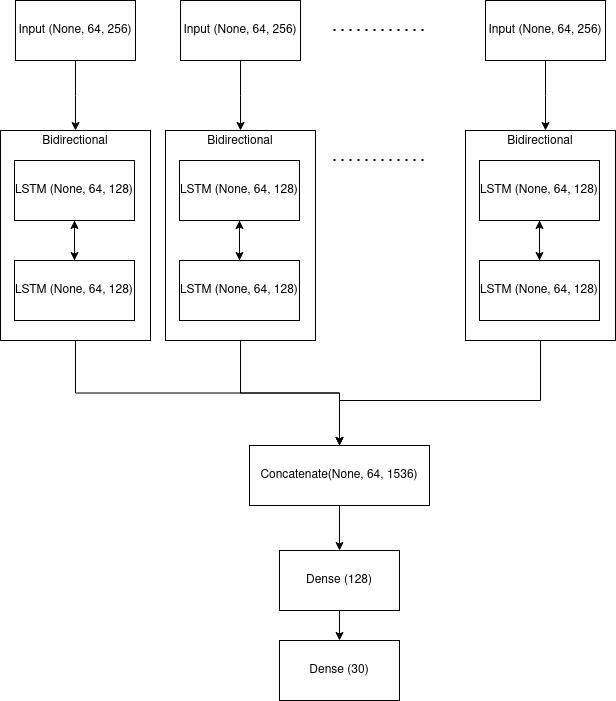
\includegraphics[width=0.70\linewidth]{sp-con-arch.png}
    \caption{Architektura hierarchicznego modelu czasowego opartego o cechy RGB uczestników akcji, ze zrównolegloną warstwą dwukierunkową LSTM oraz warstwą konkatenacji}
    \label{fig:sp-con-arch}
\end{figure}

\subsubsection{Wyniki}
Hierarchiczne modele oparte na cechach RGB osiągnęły skuteczności 62.48\%, 69.38\% wyliczone w tabeli \ref{tab:hier-rgb-wyniki}. Zastąpienie cech szkieletowych cechami RGB dało wysoką poprawę rzędu 20 punktów procentowych. Model ten rozwiązuje część problemów, które występują dla danych szkieletowych, posiada informację o ruchach poszczególnych osób, oraz części obrazu, jednak nie posiada informacji o tle oraz miejscu wykonywanej akcji. 

Wyniki uzyskane przez model wykorzystujący warstwę Max-Pooling'u są zbliżone do wyników, które uzyskał Ibrahim et al. \cite{Ibrahim2015} dla trudniejszego zbioru, które wynoszą 51.1\%. Zastąpienie warstwy Max-Pooling'u warstwą konkatenacji, oraz zepchnięcie dwukierukierunkowej warstwy LSTM do analizy akcji pojedynczych osób poprawiło skuteczność modelu o około 8 punktów procentowych, potwierdzając hipotezę o bardzo dużej utracie danych związanych z redukcją wymiaru. 
\begin{table}[!h] \centering
\caption{Wyniki modelów hierarchicznych opartych na cechach RGB}
\begin{tabular} {| c | c | c | c | r |} \hline
    Model & Podział 1.  & Podział 2. & Podział 3. & \textbf{Średnia} \\ \hline\hline
    Hierarchiczny model RGB &  61.42\%	& 62.47\%	& 63.56\%	& \textbf{62.48\%} \\ \hline
    Hierarchiczny model RGB z konkatenacją &  68.82\%	& 68.58\%	& 70.74\%	& \textbf{69.38\%} \\ \hline
\end{tabular}
\label{tab:hier-rgb-wyniki} 
\end{table}

\subsection{Model badający cały obraz}
Przeprowadzone również zostały eksperymenty modelu działającym na całych klatkach nagrania, bez wyznaczania poszczególnych osób. Wejściem do modelu jest sekwencja długości $T$, uzyskana w sposób opisany w rozdziale \ref{sekwncje-klatek}. Wejście przekazywane jest dwukierunkowej sieci LSTM, takiej samej jak we wszystkich wcześniej przedstawionych modelach, następnie do dwóch warstw gęstych oraz warstwy klasyfikacyjnej. Architektura przedstawiona została na rysunku \ref{fig:frame-arch}. Całkowita liczba trenowalnych parametrów modelu wynosi 435 710. 
\begin{figure}[!h]
    \centering 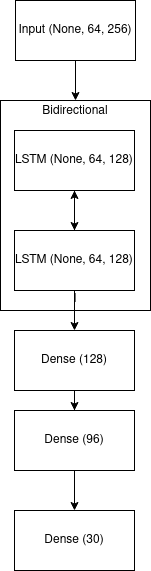
\includegraphics[width=0.2\linewidth]{frame-arch.png}
    \caption{Architektura modelu czasowego opartego o cechy RGB klatek nagrania}
    \label{fig:frame-arch}
\end{figure}
\subsubsection{Wyniki}
Model badający cały obraz osiągnął skuteczność 76.16\%, wyliczone w tabeli \ref{tab:frame-rgb-wyniki}. Wynik ten udowadnia, że  globalne cechy obrazu niosą więcej informacji niż same akcje poszczególnych osób na nagraniu. 
\begin{table}[!h] \centering
\caption{Wyniki}
\begin{tabular} {| c | c | c | c | r |} \hline
    Model & Podział 1.  & Podział 2. & Podział 3. & \textbf{Średnia} \\ \hline\hline
    Model klatkowy &  78.10\%	& 74.88\%	& 75.49\%	& \textbf{76.16\%} \\ \hline
\end{tabular}
\label{tab:frame-rgb-wyniki} 
\end{table}
\subsection{Fuzja modeli} 
Dysponując dużą liczbą modeli, działających na różnych cechach przetestowane zostało również wielomodelowe rozwiązanie problemu poprzez dokonanie późnej fuzji modeli, które osiągnęły najlepszą skuteczność dla konkretnego rodzaju danych, z modelem działającym na całym obrazie. Eksperyment ten ma na celu rozszerzenie kontekstu na jakim działa model badający cały obraz o więcej informacji o akcjach poszczególnych osób. Badane modele razem z wynikami przedstawione zostały w tabeli \ref{tab:fuzja-wyniki}. 

Późna fuzja wykonana została poprzez odrzucenie z łączonych ze sobą modeli ostatniej warstwy gęstej (głowy modelu), oraz konkatenację wyjściowych logitów z wyjściowej warstwy gęstej i przekazanie ich do nowej głowy modelu (warstwy gęstej o liczbie neuronów równej liczbie klas). Na rysunku \ref{fig:fuse-example-arch} przedstawiona została fuzja modelu działającego na całych klatkach \ref{fig:frame-arch} z modelem hierarchicznym \ref{fig:sp-con-arch}. Połączone ze sobą modele trenowane są w całości od nowa. 


\begin{figure}[!h]
    \centering 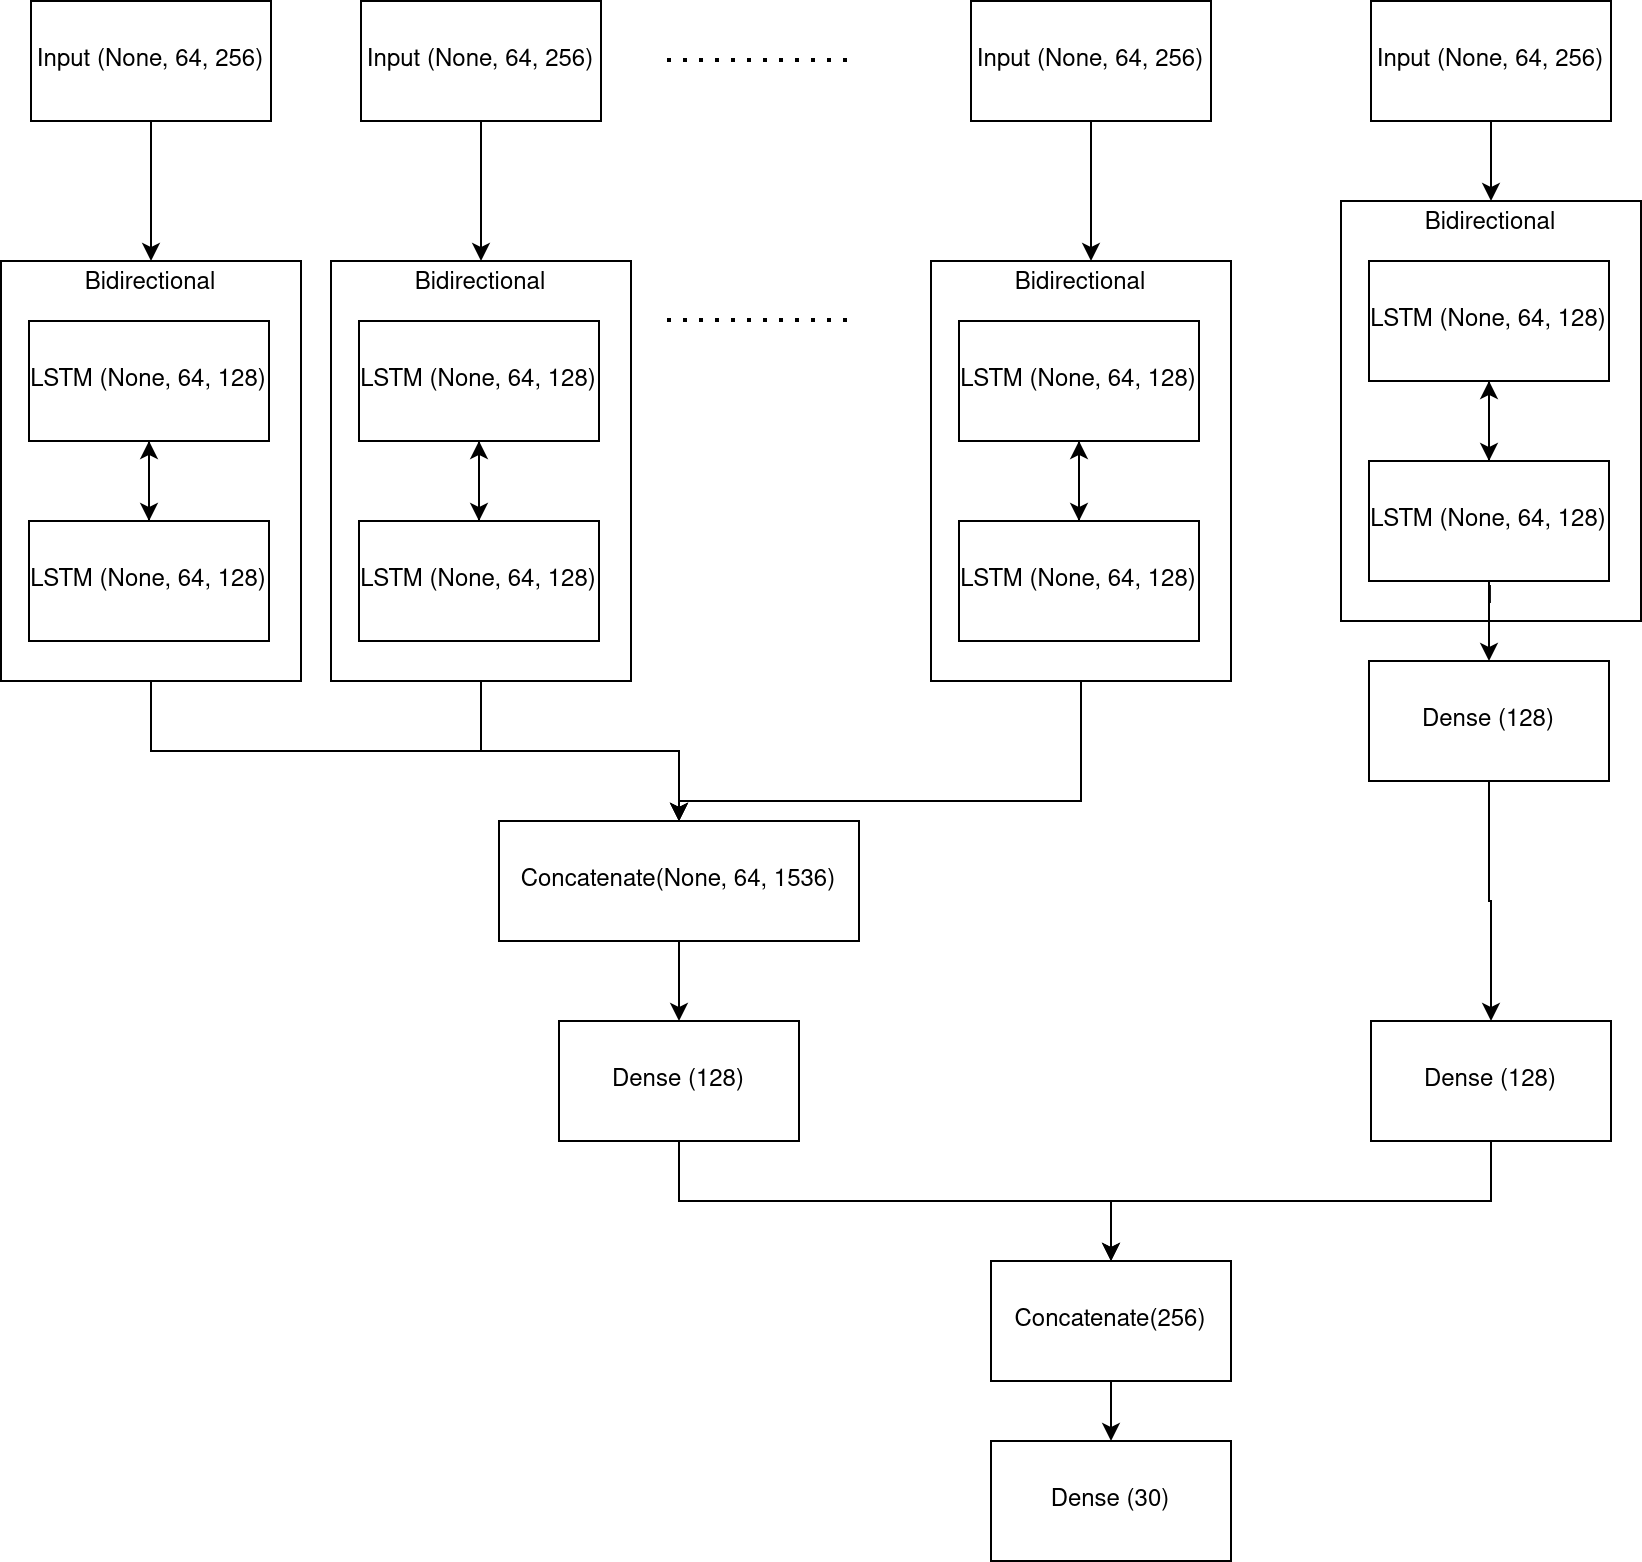
\includegraphics[width=0.70\linewidth]{fuse-example.png}
    \caption{Architektura hierarchicznego modelu czasowego opartego o cechy RGB uczestników akcji, ze zrównolegloną warstwą dwukierunkową LSTM oraz warstwą konkatenacji}
    \label{fig:fuse-example-arch}
\end{figure}

\subsubsection{Wyniki} \label{najlepszy-model}
Wyniki fuzji z konkretnymi modelami zostały przedstawione w tabeli \ref{tab:fuzja-wyniki}. 

Fuzja modelu szkieletowego z modelem klatkowym daje pomijalną poprawę wynoszącą około 1 punktu procentowego. Niski poziom poprawy spowodowany jest prawdopodobnie niską skutecznością samego modelu szkieletowego, która została wykazana we wcześniejszym eksperymencie. Najprawdopodobniej model w dużej mierze ignoruje wkład szkieletowy oraz predykcji dokonuje wzorując się tylko na klatkach nagrania. 

Fuzja modelu hierarchicznego opartego na cechach RGB z modelem klatkowym przyniosła wysoką poprawę wynoszoną około 5 punktów procentowych. W tym przypadku model zgodnie z wcześniej postawioną hipotezą, korzysta z rozszerzonego kontekstu. Jest to również model o najlepszej skuteczności opisany w tej pracy. Zostanie wykorzystany do porównań z modelami referencyjnymi na tym zbiorze. 

Fuzja wszystkich trzech modelów daje statystycznie nieistotny rezultat w porównaniu do fuzji hierarchicznego modelu RGB oraz modelu klatkowego. Fuzja z modelem szkieletowym nie daje istotnej poprawy skuteczności. 
\begin{table}[!h] \centering
\caption{Wyniki modeli po fuzji.}
\begin{tabular} {| c | c | c | c | r |} \hline
    Model & Podział 1.  & Podział 2. & Podział 3. & \textbf{Średnia} \\ \hline\hline
    \begin{tabular}[c]{@{}l@{}}Hierarchiczny model szkieletowy +\ \ \ \ \ \ \ \ \ \ \ \ \ \ \ \ \ \\ Model klatkowy\end{tabular} &  77.82\%	& 76.18\%	& 78.19\%	& \textbf{77.40\%} \\ \hline
    \begin{tabular}[c]{@{}l@{}}Hierarchiczny model RGB z konkatenacja +\\ Model klatkowy\end{tabular} &  82.65\%	& 79.24\%	& 79.68\%	& \textbf{80.53\%} \\ \hline
    \begin{tabular}[c]{@{}l@{}}Hierarchiczny model szkieletowy +\\ Hierarchiczny model RGB z konkatenacja +\\ Model klatkowy\end{tabular}&  80.76\%	& 78.78\%	& 81.27\%	& \textbf{80.27\%} \\ \hline
\end{tabular}
\label{tab:fuzja-wyniki} 
\end{table}
\subsection{Interpretacja wyników modelu} 
W tej sekcji opisana została interpretacja wyników zwracanych przez najlepszy znaleziony model w eksperymentach 
\ref{najlepszy-model}. Macierz pomyłek modelu przedstawiona została na rysunku \ref{fig:conf-matrix}. Model skutecznie 
nauczył się rozpoznawać większość klas. Najbardziej problematyczne sporty zostały opisane poniżej.
\begin{figure}[!h]
    \centering 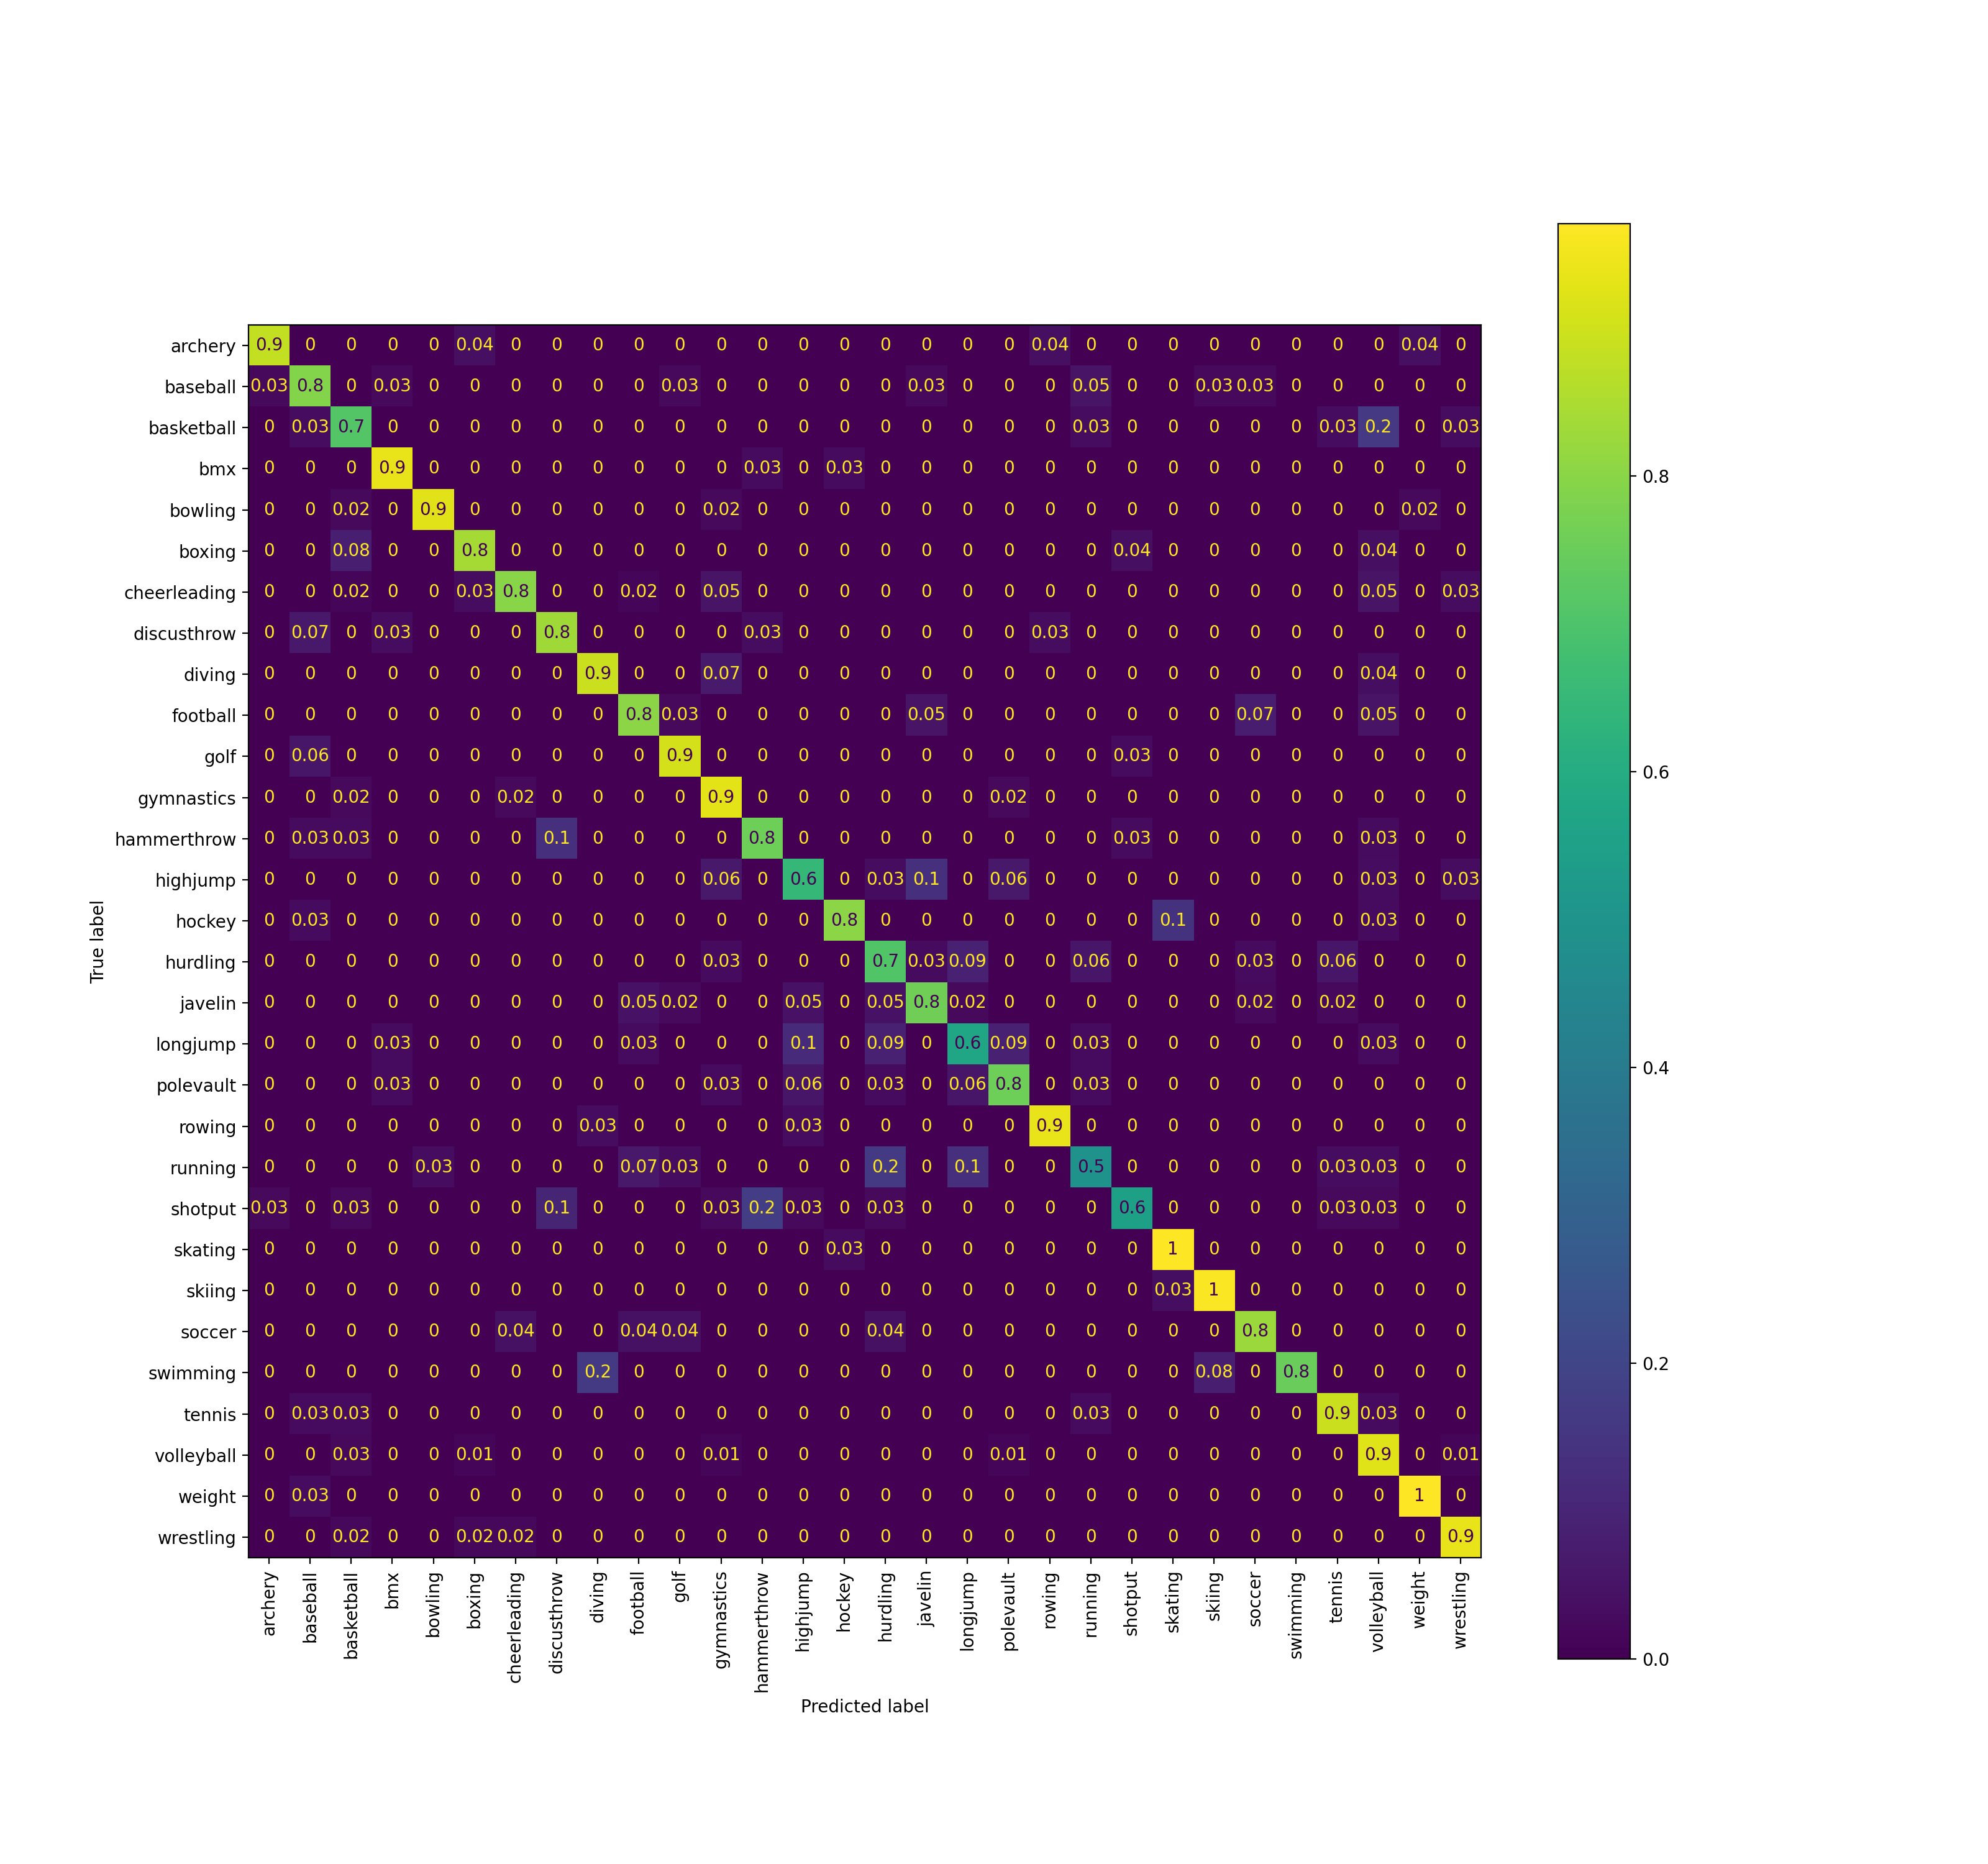
\includegraphics[width=0.99\linewidth]{confusion_matrix.png}
    \caption{Macierz pomyłek najlepszego znalezionego modelu}
    \label{fig:conf-matrix}
\end{figure}
\subsubsection{Wariacje biegania} 
Model ma największy problem z rozpoznawaniem sportów będącymi wariacjami biegania np. bieg przez płotki oraz sportami,
których dużą częścią jest wykonanie rozbiegu np. skok w dal. W pierwszym przypadku model ma problem z rozpoznawaniem 
innej techniki biegu. Drugim problemem jest zastosowanie próbkowania nagrań wideo opisanego w sekcji 
\ref{klasyfikacja}. Dla sportów tj. skok w dal, w których dużą część stanowi wzięcie rozbiegu większość próbek, 
będzie klasyfikowana jako bieg, a część kluczowa, czyli sam skok stanowi mniejszość próbek, przez co nie będą one w 
stanie stanowić przeciwwagi dla wcześniejszych predykcji. 
\subsubsection{Rzuty}
Kolejnym widocznym problemem modelu są rzuty tj. rzut kulą, rzut młotem, rzut dyskiem. Problem rozpoznania tych klas 
wynika z bardzo zbliżonej techniki wykonywanego sportu oraz otoczenia, w jakim wykonuje się sport, czyli klatki z siatki. 
\subsubsection{Koszykówka - Siatkówka}
Pomyłki modelu dla tych dwóch kategorii najprawdopodobniej wynikają z rodzajów boiska, 
na którym wykonywany jest sport oraz podobnych ruchów wykonywanych przez zawodników. W dużej mierze nagrania wchodzące 
w skład zbioru danych przedstawiają treningi wykonywane na sali gimnastycznej przygotowanej do ogólnego użytku (w tle 
znajdują się rozwieszone kosze do gry w koszykówkę). Część ruchów wykonywanych przez zawodników w tych sportach jest 
również bardzo podobna, a nawet taka sama np. blok.   
\newpage
\section{Zestawienie wyników}
Zbiór \textit{"Sports videos in the wild"} \cite{svw} został szeroko zbadany przy użyciu wielu metod. W tym rozdziale dokonane zostaje porównanie wyniku uzyskanego w przeprowadzonych eksperymentach z wynikami uzyskanymi innymi metodami na tym zbiorze danych. 
\subsection{Metryki bazowe}
\subsubsection{Bazowa metryka zbioru SVW}
Twórcy zbioru SVW \cite{svw} dostarczają razem ze zbiorem kilka metryk bazowych. Najlepszy wynik uzyskują stosując algorytm gęstych trajektorii wykorzystujący histogram zorientowanych gradientów (HOG). Proces rozpoczyna się od gęstego próbkowania punktów na kolejnych klatkach wideo, co oznacza, że punkty są wybierane z dużą gęstością w całym kadrze, a nie tylko na podstawie wybranych punktów charakterystycznych. Dzięki temu, gęste trajektorie mogą przechwycić bardziej precyzyjne informacje o ruchu wideo, zwłaszcza w obszarach o szybkim i skomplikowanym ruchu.

Następnie algorytm oblicza cechy dla każdego próbkowanego punktu, które zawierają informacje o intensywności, kierunku i ewolucji ruchu w sąsiedztwie danego punktu. Informacje te reprezentowane są przez Histogramy zorientowanych Gradientów (HOG). W rezultacie otrzymywany jest zestaw cech, które opisują lokalne wzorce ruchu na różnych obszarach wideo.

Kolejnym etapem jest śledzenie trajektorii, czyli określenie przemieszczenia próbkowanych punktów na kolejnych klatkach. Wykorzystane zostały tu techniki estymacji przepływu optycznego, które pozwalają na śledzenie ruchu pikseli w czasie. 

Ostatnim elementem algorytmu jest uwzględnienie informacji czasowej, czyli ewolucji ruchu wideo. Trajektorie są grupowane w sekwencje, a następnie budowane są trajektorialne deskryptory, które przechwytują zmiany w ruchu na przestrzeni czasu.

Zastosowanie tego algorytmu na zbiorze daje skuteczność wynoszącą \textbf{61.53\%}. 

\subsubsection{Dostrajanie modelu Inception-Resnet-V2}
Joey Asperger et al. \cite{cnn-joey} wykonuje w swojej pracy wyczerpujące testy wykorzystujące sieci splotowe oraz ich kombinacje z warstwami LSTM. Najlepsze wyniki osiąga poprzez dostrojenie wszystkich warstw modelu Inception-Resnet-V2 \cite{inception-resnet-v2}, głębokiej sieci neuronowej, który łączy koncepcje dwóch popularnych architektur: Inception i ResNet. Wykorzystuje on zalety obu modeli, takie jak wieloskalowe ekstrakcje cech, połączenia residualne i globalne uśrednianie pooling, aby osiągnąć wyjątkową skuteczność w zadaniach przetwarzania obrazów. 

W pracy najlepsze wyniki osiąga na uśrednionych, równomiernie rozłożonych w wideo 10 klatkach, wynoszące \textbf{75.9\%}. Połączenie modelu Inception-Resnet-V2 z warstwą LSTM dało wyniki bardzo zbliżone do wyników uzyskanych w tej pracy, dla modelu opartego wyłącznie na całych klatkach oraz warstwie LSTM \ref{fig:frame-arch} wynoszącą 74.7\%. 

\subsubsection{Rozszerzenie modelu VGG16}
Santanu Datta \cite{kumar} w swoich eksperymentach rozszerza model VGG16 \cite{vgg16} o dodatkowe warstwy splotowe oraz głębokie. Model VGG16 składa się z 16 warstw, które składają się głównie z konwolucyjnych warstw neuronowych (Convolutional Neural Networks - CNN) i warstw poolingowych, zakończonych pełnopowiązkowymi warstwami ukrytymi i wyjściowymi. Jego główną cechą jest prostota architektury, w której stosuje się niewielkie jądra filtrów (3x3 piksele) w wielu kolejnych warstwach, co pozwala na głębokie i skuteczne przetwarzanie obrazów. 

W eksperymentach próbkowane są 4 klatki nagrania, którch reprezentacje uzyskane są przez infrencje wytrenowanego modelu VGG16. Reprezentacje są konkatenowane do wspólnego wektora, który trafia do warstwy splotowej 3D, dwóch warstw głębokich oraz warstwy wyjściowej.

Wynik, który został uzyskany na zbiorze SVW \cite{svw} wynosi \textbf{74.56\%}. 
\subsection{Porównanie wyników}
W tabeli \ref{tab:result-comp} przedstawione zostały zbiorcze wyniki modelów opisanych w tym rozdziale. Zaproponowany w tej pracy model osiągnął najwyższą skuteczność. Można zauważyć, że modele oparte wyłącznie na sieciach splotowych oraz całych klatkach osiągnęły bardzo zbliżoną skuteczność, co jest spodziewanym wynikiem. Dopiero rozszerzenie modelu o dodatkowe cechy daje zauważalną zmianę w okolicach 5 punktów procentowych. 

Najgorszy wynik uzyskała metoda gęstych trajektorii, udowadniając, że metody oparte na ręcznym projektowaniu cech wejściowych do modelu odstają skutecznością od uczenia głębokiego dla tak mocno skomplikowanych problemów. 
\begin{table}[!h] \centering
\caption{Porównanie wyników}
\begin{tabular} {| c | c | c | c | r |} \hline
    Model & Wynik \\ \hline\hline
    \begin{tabular}[c]{@{}l@{}}\textbf{Hierarchiczny model RGB z konkatenacją + Model klatkowy}\end{tabular} & \textbf{80.53\%} \\ \hline
    \begin{tabular}[c]{@{}l@{}}Model klatkowy\end{tabular}&  76.16\% \\ \hline
    \begin{tabular}[c]{@{}l@{}}Dostrojony model Inception-Resnet-V2\end{tabular}&  75.9\% \\ \hline
    \begin{tabular}[c]{@{}l@{}}Rozszerzony model VGG16\end{tabular}&  74.56\% \\ \hline
    \begin{tabular}[c]{@{}l@{}}Gęste trajektoria\end{tabular}&  61.53\% \\ \hline
\end{tabular}
\label{tab:result-comp} 
\end{table}
\subsection{Problemy zastosowanego podejścia}
Rozszerzenie cech klatkowych o cechy aktywności pojedynczych osób, pomimo znaczącej poprawy względem bazowych modeli wiąże się z kilkoma znaczącymi wadami. 
\subsubsection{Wstępne przetworzenie danych}
Dodanie cech aktywności pojedynczych osób do modelu wymaga dużo większej ilości wstępnego przetworzenia danych. Przede wszystkim wymagana jest inferencja detektora znajdującego osoby na nagraniu oraz przetwarzanie znajdujące kluczowych uczestników. Następnie wymagane jest zakodowanie ich cech przez sieć splotową, łącznie dając dodatkową liczbę inferencji równej liczbie badanych osób na nagraniu.

Konieczność zastosowania tak złożonego przetworzenia danych wyklucza model z zastosowania go do wykonywania predykcji na bieżąco, nadaje się wyłącznie do przetwarzania gotowych nagrań. 
\subsubsection{Rozmiar modelu}
Dołączenie hierarchicznej części modelu do modelu opartego wyłącznie na klatkach ma bardzo duży wpływ na liczbę parametrów sieci, rozmiar modelu po zastosowaniu fuzji rośnie ponad 2 krotnie, z czym wiąże się większy czas inferencji modelu oraz czas treningu. Porównanie tych parametrów zostało przedstawione w tabeli \ref{tab:param-comp}. 
\begin{table}[!h]  \centering
\caption{Porównanie parametrów modeli}
\begin{tabular} {| c | c | c | c | r |} \hline
    Model & Liczba trenowalnych parametrów  & Czas inferencji& Czas treningu\\ \hline\hline
    Model klatkowy &  435 710	& 6 ms	& 61 s  \\ \hline
    Model hierarchiczny &  1 017 950	& 50 ms	& 526 s \\ \hline
\end{tabular}
\label{tab:param-comp}
\end{table}
\subsubsection{Zaszumione nagrania wideo}
Zarówno w testowanym zbiorze danych, jak i przy realnych zastosowaniach modelu mogą wystąpić nagrania, w których detekcja osób zawiedzie, na przykład ze względu na zbyt małą rozdzielczość nagrania, lub algorytm selekcji osób nie wybierze osoby faktycznie wykonującą aktywność, i skupi się na osobach otaczających. W takich przypadkach zastosowanie hierarchicznej części modelu może nie mieć żadnego skutku (otrzyma na wejściu same 0), lub nawet pogorszy wyniki skupiając się na tłumie. Zatem jednym z warunków aby fuzja modeli dała skuteczną poprawę, jest stosowanie modelu na nagraniach, na których jakość detekcji osób jest wystarczająco wysoka.   
\newpage
\section{Podsumowanie}
\subsection{Omówienie}
W pracy przedstawione zastosowania hierarchicznych modeli LSTM w zadaniu rozpoznawania dyscypliny sportu na podstawie materiałów wideo. Przetestowane zostały modele działające na różnych cechach wejściowych: 
\begin{itemize}
    \item Sylwetkach reprezentowanych poprzez punkty na stawach i kluczowych fragmentach ciała sportowców
    \item Cechach RGB pojedynczych osób
    \item Cechach RGB całych klatek. 
\end{itemize}
Cechy RGB wyekstrahowane zostały przy pomocy modelu MobileNetV3. 
Dokonana została również fuzja kombinacji modeli z klasycznym modelem opartym na cechach RGB całej klatki. Najlepszą skuteczność wynoszącą 80.53\%, osiągnęła fuzja modelu opartego na cechach RGB pojedynczych osób z modelem opartym na całych klatkach.
\subsection{Napotkane problemy}
\subsubsection{Wybranie osób do modelu hierarchicznego}
Jako, że przy zastosowanym podejściu rozpoznawanie dyscypliny sportu staje się klasyfikacją aktywności grupowej, w pracy musiał zostać rozwiązany problem doboru osób na wejście modelu. Naturalnym podejściem byłoby wzięcie wszystkich możliwych osób, jednak takiego modelu nie dałoby się trenować w całości oraz mogłoby to wprowadzić duży nakład pracy, która mogłaby nie dać pozytywnych efektów, na przykład gdyby na wejściu do modelu podana zostałaby cała widownia dużego wydarzenia sportowego. Wartość ta nie może być również dowolnie duża ze względu ograniczeń technicznych. Dla modelu, działającego na cechach RGB pojedynczych osób, dodanie osoby liniowo zwiększa rozmiar zbioru danych treningowych oraz czas treningu. Z tego względu w pracy została wybrana stała, maksymalna dla sprzętu, na którym prowadzone były badania wartość równa 6. 
\subsubsection{Przetrenowanie modeli}
Nadmiarowe dopasowanie modelu do danych treningowych może wystąpić przy zbyt długim treningu, dużą rozbieżnością między zbiorem treningowym oraz walidacyjnym, lub przy zbyt obszernym modelu. W pracy problemy te zostały rozwiązane kolejno poprzez zastosowanie funkcji wcześniejszego przerwania treningu, zastosowanie warstw dropout, możliwie najlepsze uogólnienie problemu oraz dobranie odpowiedniego rozmiaru architektury. Eksperymenty również wykazały, że zastąpienie pojedynczych warstw LSTM dwukierunkowymi LSTM znacznie poprawiło jakość treningu.  

\subsection{Dalsze prace}
\subsubsection{Działanie modelu na żywo}
Aktualnie wstępne przetwarzanie danych wejściowych dla modelu jest zbyt złożone aby wykonywać je w czasie rzeczywistym. Warto zbadać zachowanie rzadszego i bardziej równomiernego próbkowania, niż zostało zastosowane w tej pracy, co odciążyło by całe przetwarzanie i przyśpieszyło działanie modelu. 
\subsubsection{Zastosowanie modelu do innych aktywności}
W pracy model został przetestowany wyłącznie w zadaniu rozpoznawania dyscyplin sportu oraz pokazał, że jest w stanie przynieść w nim poprawę w porównaniu do modeli bazowych. Jako, że podejście w przetwarzaniu danych jest uniwersalne i może zostać wykorzystane do rozpoznawania dowolnych aktywności, warto przetestować, czy poprawa będzie zauważalna również dla innych zbiorów danych składających się z bardziej ogólnych aktywności.   
% \input{tex/3-code-listings} % wystarczy podmienić swoje pliki main.tex i eiti-thesis.cls
                            % na nowe wersje, a cały tekst pracy pozostaje nienaruszony.
                            
%--------------------------------------------
% Literatura
%--------------------------------------------
\cleardoublepage % Zaczynamy od nieparzystej strony
\printbibliography

%--------------------------------------------
% Spisy (opcjonalne)
%--------------------------------------------
\newpage
\pagestyle{plain}

% Wykaz symboli i skrótów.
% Pamiętaj, żeby posortować symbole alfabetycznie
% we własnym zakresie. Ponieważ mało kto używa takiego wykazu,
% uznałem, że robienie automatycznie sortowanej listy
% na poziomie LaTeXa to za duży overkill.
% Makro \acronymlist generuje właściwy tytuł sekcji,
% w zależności od języka.
% Makro \acronym dodaje skrót/symbol do listy,
% zapewniając podstawowe formatowanie.
% //AB
\vspace{0.8cm}
\acronymlist
\acronym{EiTI}{Wydział Elektroniki i Technik Informacyjnych}
\acronym{PW}{Politechnika Warszawska}

\listoffigurestoc     % Spis rysunków.
\vspace{1cm}          % vertical space
\listoftablestoc      % Spis tabel.
\vspace{1cm}          % vertical space
\listofappendicestoc  % Spis załączników

% Załączniki
% \newpage
% \appendix{Nazwa załącznika 1}
% \lipsum[1-8]

% \newpage
% \appendix{Nazwa załącznika 2}
% \lipsum[1-4]

% Używając powyższych spisów jako szablonu,
% możesz tu dodać swój własny wykaz bądź listę,
% np. spis algorytmów.

\end{document} % Dobranoc.
